\chapter{Detektoren in der Teilchenphysik}
Was wir wissen wollen:
\begin{itemize}
	\item Transversalimpuls $p_\text{T}$
	\item Polarwinkel $\phi$
	\item (Pseudo)rapidität (also Azimuthwinkel) $\eta$
	\item Energie
	\item Teilchenart.
\end{itemize}

\section{Die Blasenkammer}
Das Prinzip der Blasenkammer ist einfach:
Die Flüssigkeit (z.B. H2) im Unterdruck beginnt an Verunreinigungen und Ionisationskeimen zu sieden.
Diese Bläschen werden fotografiert.
Das ist zum einen sehr ungenau und zum anderen können wir so keine Aussagen über die Teilchenart machen.

\section{Nachweismethoden für Teilchen}
\begin{figure}
	\centering
	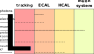
\includegraphics[width=.7\textwidth]{./img/detectorsystem.pdf}
	\caption{Verschiedene Teilchen können durch die Ebenen unterschieden werden.}
	\label{fig:detectionmethods}
\end{figure}
Um verschiedene Teilchenarten zu unterscheiden, ist ein Detektor durch mehrere Ebenen aufgebaut (siehe \autoref{fig:detectionmethods}).

\textbf{Die tracking layer} sorgt für eine Richtungsbestimmung.

\textbf{Das elektromagnetische Kalorimeter} bestimmt die Energie von Teilchen die im Wesentlichen über die elektromagnetische Kraft wechselwirken.

\textbf{Im hadronischen Kalorimeter} lassen sich Teilchen nachweisen, die überwiegend der starken Wechselwirkung unterliegen.
Da hadronische Teilchen szintillierendes Material fast ungehindert durchdringen ist der Nachweis über das em-Kalorimeter nicht gewährleistet.

\textbf{Im Myon-System} werden die hochenergetischen Myonen nachgewiesen, da sie für einen Nachweis im em-Kalorimeter zu hochenergetisch sind.

\section{Spurdetektoren}

\section{Kalorimeter}

\subsection{Elektromagnetische Schauer}

\subsection{Hadronische Schauer}

\section{Das Myon-System}
